\section{Modelling ``Optimize a Data Center''} \label{section:data-center}

In this section, we will analyze the model developed for the Hash Code 2015
qualification round problem, titled "Optimizing a Data Center." To begin, in
Section~\ref{section:data-center-problem}, we will provide a comprehensive
description of the problem and key concepts outlined in the problem statement,
which are essential for understanding the context. In Section~\ref{section:
  data-center-model}, we will delve into the model developed for this problem,
highlighting the representation, objective function, bounds, and heuristic
construction of solutions from both a theoretical and practical perspective,
taking into account the framework proposed by Vieira et al.\cite{vieira2009uma}
and the practical implementation contained in the API for constructive search by
Outeiro et al.\cite{outeiro2021application}. Finally, in Section~\ref{section:
  data-center-results}, we will present a brief overview of the results and in
Section~\ref{section:data-center-remarks}, we will offer some final thoughts and
observations on the problem and the model developed for it.

\subsection{Problem Description} \label{section:data-center-problem}

As previously discussed in Section~\ref{section:hashcode2015-qualification},
the problem at hand entails optimizing the placement of servers in a data center.
The data center is modeled as a series of rows, each containing a number of
slots in which servers can be placed. However, it should be noted that certain
slots may be unavailable due to other installations within the data center. The
servers available are characterized by a tuple containing both size, measured in
slots, and computing capacity. Furthermore, servers are logically divided into
pools, to which they can contribute their capacity, with the capacity of the
pool being defined as the sum of the capacities of the servers assigned to it.

\begin{figure}[h] \centering 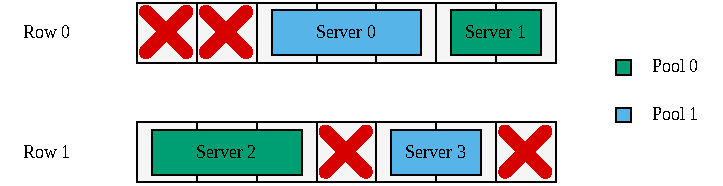
\includegraphics[width=0.9\textwidth,
    keepaspectratio]{../assets/dc/dc-example.pdf} \caption{Example Data Center
    Layout} \label{fig:data-center-layout} \end{figure}

\begin{table}[ht] \centering \begin{tabular}{ccc} \toprule Server & Size &
               Capacity                       \\ \midrule 0 & 3 & 2 \\ 1 & 2 & 5 \\ 2 & 3 & 10 \\ 3 & 2 & 3 \\
               \bottomrule\end{tabular} \caption{Server Properties} \label{table:
    dc-example-properties} \end{table}

As an illustration the figure~\ref{fig:data-center-layout} provides an overview
of a possible data center layout. In this particular case the data center is
composed by 2 rows containing a total of seven slots each where in both cases
only 5 are available for positioning of servers. Moreover the servers placed
were assigned to two distinct resource pools.

\begin{definition}[Guaranteed Capacity] \label{definition:guaranteed-capacity}
  Given a resource pool $p$, the guaranteed capacity $gc_{p}$ is a measure of the
  remaining computing capacity available in the event that at most one arbitrary
  row ($r\in\mathcal{R}$) of the data center becomes offline. This can be formally
  defined as follows: \begin{equation} {gc}_{p} = \min_{r \in \mathcal{R}}
    ({\sum_{s \in p} c_{s}} - {\sum_{s \in p \wedge s \in r} c_{s}}) \end{equation}
\end{definition}

Given the representation of a possible layout of a data center, the objective
of this problem can be succinctly defined as finding an optimal placement of
servers in the rows and assigning them to pools, with the goal of maximizing the
guaranteed capacity~\ref{definition:guaranteed-capacity}, of all resource pools
present in the data center. Formally, this objective can be described by the
equation shown in~\ref{definition:dc-objective}.

\begin{definition}[Objective Function] \label{definition:dc-objective} Given a
  set of pools $\mathcal{P}$, the objective function for an instance of this
  problem is defined as: \begin{equation} f(s) = \min_{p \in \mathcal{P}}
    ({gc}_{p}) \end{equation} \end{definition}

The objective function value resulting from the evaluation of a solution is,
from a contestant's perspective, the score that will be obtained for solving a
particular problem instance. As an example, consider the data center layout
shown in Figure~\ref{fig:data-center-layout} and the server properties displayed
in Table~\ref{table:dc-example-properties}.

\begin{table}[ht] \centering \begin{tabular}{@{\extracolsep{4pt}}cccc} \toprule
    Pool & Row 0 & Row 1 & Guaranteed Capacity \\ \midrule 0 & 5 & 10 & 5 \\ 1 & 2 &
    3    & 2                                   \\ \bottomrule\end{tabular} \caption{Guaranteed Capacities For Each Pool
    In Example~\ref{fig:data-center-layout}} \label{table:dc-gc-example} \end{table}

In this scenario, the score of the server placement, as determined by the
evaluation of the objective function~\ref{definition:dc-objective}, would be
$\min (5, 2) = 2$. The table shown in~\ref{table:dc-gc-example} illustrates the
calculation of the guaranteed capacities for this example.

Regarding the instances, the problem statement guarantees that the generated
instances along with the description of the unavailable slots and the servers to
be placed will have the following properties:

\begin{itemize} \item $ 1 \leq \mathcal{R} \leq 1000$: Denotes the number of
        rows in the data center. \item $ 1 \leq \mathcal{S} \leq 1000$: Denotes the
        number of slots in a row. \item $ 0 \leq \mathcal{U} \leq \mathcal{R} \times
          \mathcal{S}$: Denotes the number of unavailable slots. \item $ 1 \leq
          \mathcal{P} \leq 1000$: Denotes the number of resource pools to be created.
  \item $ 1 \leq \mathcal{M} \leq \mathcal{R} \times \mathcal{S}$: Denotes the
        number of servers to be allocated. \end{itemize}

On a final note, it is required that contestants generate a solution that
includes an ordered list of servers, specified by the problem instance, where
each server is assigned a row, pool, and starting slot (position) in the
selected row. This information is critical to the modeling process, as it
affects the representation of the problem, solutions, and components mainly from
an implementation perspective.

\subsection{Model} \label{section:data-center-model}

In this section, we will proceed to define the model for this problem.
Specifically,we begin by addressing key aspects such as the instance parameters
and the representation of this problem. Subsequently, we will delve into the
representation of solutions, the ground sets, and the components of this problem.
We will then present the objective function, giving particular attention to how
solutions are evaluated within the context of our chosen representation. We will
also explore the bounds established for this problem. Finally, we will discuss
the heuristics and heuristic rules that are utilized to construct solutions.

It should be noted that the effort of modeling will be formulated within the
context of the API for constructive search developed by
Outeiro~\cite{outeiro2021application}. As such, the modeling will be described
using the concepts and terminology specified in said work.

\subsubsection{Instance Parameters} \label{section:data-center-representation}

For the purpose of capturing the relevant information pertaining to the problem
at hand, we initiated the process by defining the \texttt{Problem} data
structure. This structure, in the context of modeling, encompasses the essential
attributes of the instance that are required for, among other things, the
construction of solutions. However, prior to specifying the data that was stored
for the problem, it is necessary to provide clarification regarding the terms
``segment'' and ``server''.

During the modeling phase, we identified that the rows of the data center could
not be considered as a sort of ``standard knapsack'', where placing a server
would simply encompass the consumption of available slots. This is because the
presence of unavailable slots in the row may prevent a server with a given size
from being placed. Thus, a row having sufficient space to accommodate a server
is not a sufficient requirement for its placement. Instead, we can view each row
of the data center as a collection of multiple knapsacks, where each group of
consecutive available slots is considered as a separate knapsack, which we refer
to as a segment.

From a modelling perspective, a segment can be then be described as a tuple
containing three defining fields. The first is the \textit{size}, which pertains
to the number of available slots. The second is the \textit{row}, which
obviously represent the row where that segment belongs. And last, the the
\textit{start}, which represents the starting slots (position) for the segment
in that rows since it useful in the solution construction.

Furthermore, as previously mentioned, a server has two properties: the
\textit{size} and the \textit{capacity}. From a modeling perspective, these are
the fields of a tuple that defines the server, with the added \textit{id} that
serves as an indexing reference in our representation.

Having defined the terminology, our solution structure is comprised of the
following fields:

\begin{itemize} \item \textbf{pools}: A numerical value indicating the quantity
        of resource pools to be created. \item \textbf{servers}: An list of servers to
        be allocated to segments and resource pools. \item \textbf{sorted (servers)}: A
        list containing, indexes of the servers sorted by an heuristic (ratio between
        the size and capacity of the server). This is used in the solution-building
        process. \item \textbf{segments}: An list of segments within the data center, to
        be populated with servers. \item \textbf{rows}: An list of sets, each of which
        records the segments associated each row. \end{itemize}

\subsubsection{Decision Space} \label{section:data-center-decision-space}

Having defined the problem the next step in the modelling process is to define
the decision space. Namely the components and the solutions.

Given that the objective of this problem is to construct a data center layout
by positioning servers in rows and assigning them to resource pools, it can be
inferred that a solution will consist of a list of objects (components) that
record this information. As such the component structure for this problem can be
defined as follows by the following properties.

\begin{itemize} \item \textbf{server}: The index (as represented in the
        "servers" list) of the selected server. \item \textbf{segment}: The index (as
        represented in the "segments" list) of the segment where the selected server
        will be placed. \item \textbf{pool}: The resource pool to which the selected
        server is to be assigned. \end{itemize}

Thus, the ground set $\mathcal{G}$ of the problem becomes defined as the set
containing tuples that represent all possible combinations of these properties.

In regards to the representation of solutions, it is important to note that in
this problem, a partial solution, which is defined as a solution in which not
all available servers have been assigned, is a feasible solution that can be
properly evaluated through the objective function. With that in mind, the model
represents solutions as structures containing the following properties:

\begin{itemize} \item \textbf{score}: The value resulting from the evaluation
        of this solution through the objective function. \item \textbf{allocation}: A
        list of components mapping a server to a given pool and segment. \item
        \textbf{gc}: A list containing the guaranteed capacities of each resource pool.
  \item \textbf{capacity}: A matrix containing the capacities of each resource
        pool for each row of the data center. \item \textbf{sc}: The remaining space in
        each segment. \end{itemize}

Additional properties, such as iterators and collections containing items
ordered by multiple criteria, are also stored in the solution. This is done in
order to maintain the state of the solution and to cache results from previous
computations, thereby improving performance. However, these properties are not
included in the present discussion, as they are not essential for a proper
understanding of the modeling process and are considered to be implementation
details.

\subsubsection{Objective Function} \label{section:
  data-center-objective-function}

As previously discussed in Section~\ref{section:data-center-problem}, the
objective function for this problem can be calculated in a similar fashion by
determining the minimum value within the range of values contained in the list
designated as ``\textit{gc}''. The method of constructing the solutions ensures
that this list is continuously updated throughout the construction process.
However, if the solution remains unmodified, the objective function value for a
given solution can be accessed efficiently through the "score" attribute defined
in the solution's model.

\subsubsection{Bound} \label{section:data-center-bound}

In contrast to the objective function, which serves as a metric for the quality
of a solution within a given context, the bounds provide insight into the
potential of a solution in the future.

In the context of this problem, where the objective is to address a bottleneck
(objective function), it is intuitive that achieving optimal solutions requires
distributing the servers for a given pool as evenly as possible across the rows
of the server. This is because in the event of a failure, it would be
detrimental if all the servers for a pool were located in the same row that
failed. Therefore, this factor was taken into consideration when formulating the
bounds.

Additionally, certain relaxations were made to the constraints of the problem
when calculating the bound. Specifically, the bound disregards the requirement
that the servers must fit within the total space available in the segments, and
only takes into account the available space in the slots for each row and the
size of the server to be placed.

Taking this into account, the upper bound for this model can be calculated in
two steps:

% Prove that this bound works (TODO) \begin{enumerate} \item \textbf{Row-Wise
Bound} \\ Let, \begin{itemize} \item $\Theta_{\mathcal{R} \setminus r}$: Denote
        the remaining empty space in all the rows in the data center but the row $r$.
  \item $\sum_{\Theta_{\mathcal{R} \setminus r}}$: Denote the maximum sum of the
        capacities of the available servers that can be fractionally placed into
        $\Theta_{\mathcal{R} \setminus r}$ w.r.t to the ratio between the capacity and
        the size of the server. This related to with a classical upper bound for the
        multiple-knapsack problem~\cite{martello1981bound}. \end{itemize} Then, The
row-wise upper bound is expressed by: \begin{equation} \Phi_{ub}^{r} =
  \frac{\sum_{\Theta_{\mathcal{R} \setminus r}}}{\mathcal{P}} \end{equation} \item
\textbf{Upper bound}\\ The upper bound for a given solution $s$ can then be
calculated as: \begin{equation} \Phi_{ub}(s) = \min_{r \in \mathcal{R}}
  \Phi_{ub}^{r} \end{equation} \end{enumerate}

Furthermore, we can apply a correction to tighten each row-wise upper bound by
discarding pools and servers that already have a guaranteed capacity, when
dropping that row, greater than the value of the row-wise upper bound. After
discarding them, we can recompute the bound for a reduced server set and number
of pools. We repeat this process until no further correction can be applied, i.e.
until no considered pool has a guaranteed capacity greater than the bound.

\subsubsection{Construction Rules} \label{section:
  data-center-construction-rules}

Having identified and defined all of the necessary elementary components of the
model, the next step is to establish the methodology for integrating these
components into functional solutions. To accomplish this, there are certain key
concepts that must be addressed, such as enumeration and assignment/removal.

In the proposed model, enumeration is achieved through the utilization of the
\textit{enumMove} and \textit{heuristicMoveWOR} operations. These operations
function similar to iterators, continuously providing components that could be
added to a solution. The specific order in which these components are presented,
for each operation within the context of this model, is defined as follows:

\begin{itemize} \item \textbf{{\textit{enumMove}}}\\ This operation allows for
        the enumeration of all feasible components in the context of this problem. A
        feasible component could be interpreted as a component that can be added to a
        solution without violating the constraints that in this case are related to the
        available space for the placement of server given that there are no restrictions
        with respect to the assignment to resource pools.

  \item \textbf{{\textit{heuristicMoveWOR}}}\\ The operation in question enables
        the sequential enumeration of all components in a specific order, determined by
        a heuristic. This order is consistent with that specified in the
        \textit{heuristicMove} function, which enables the selection of components to be
        added based on a predefined heuristic criterion. Additionally, when a component
        is yielded during the iteration, it is no longer eligible for further
        consideration, hence the inclusion of ``WOR'' in the operation name, indicating
        that the enumeration is conducted ``without replacement''.

        The heuristic employed in this model can be succinctly characterized as a
        strategy in which the server with the most favorable capacity-to-size ratio is
        assigned to the pool with the least guaranteed capacity in the row that
        possesses the highest available space. \end{itemize}

In regards to the assignment and removal of components to and from solutions,
this is accomplished through the implementation of the \textit{applyMove}
operation. In the context of this model, the addition of a component to a
solution, denoted as ``ADD'`, involves decreasing the available space within the
segment (referred to as \textit{sc}) in which the server is placed by the size
of the server, and updating the guaranteed capacity of the associated pool
(referred to as \textit{gc} and \textit{capacity}) to reflect the inclusion of
the server. Conversely, the removal of a component, denoted as ``REMOVE'',
follows a similar process but in the opposite direction, returning the capacity
to the segment from which it was originally allocated.

\subsection{Results} \label{section:data-center-results}

From a practical perspective, the limited availability of instances for testing
was a limitation of our work. However, we were able to achieve a score of 386
points on the instance that was available, which places us at 25th in the
classification table. This was achieved without using a local search approach
and with minimal fine-tuning of the algorithms.

In fact, the algorithm used was a simple testing utility that, during the
solution construction process, enumerates the $n$ best component insertions
(moves) in a heuristic manner, and selects and stores the best one based on the
calculated value of the bound. This utility can be considered general with
respect to the model, as it was implemented in adherence to the principles of
modeling. For clarity, the pseudo-code in Algorithm~\ref{algorithm:
  enum-best-heuristic} illustrates its operation.

\begin{algorithm}[htb!] \DontPrintSemicolon \caption{Narrow Guided Heuristic
    Construction} \label{algorithm:enum-best-heuristic} \KwIn{Problem Instance
    ($\mathcal{P}$), Limit (${N}$)} \KwOut{Best solution found ($s^{*}$).} \Begin{
    $s^{*} \gets \emptyset$\; \While{True}{ \normalfont{updated} $\gets False$\;
      $s^{\prime} \gets s^{*}$\; $c^{*} \gets \emptyset$\; \For{$i = 0$
        \normalfont{to} $N$}{ $c^{\prime} \gets $ \normalfont{HeuristicMoveWOR($s^{*}$,
          \textbf{\normalfont{ADD})}}\; \normalfont{ApplyMove($c^{\prime}$, $s^{\prime}$,
          \textbf{\normalfont{ADD}})}\; \If{$\Phi_{ub}(s^{\prime})$ > $\Phi_{ub}(s^{*}$)}{
          $c^{*} \gets c^{\prime}$\; \normalfont{updated} $ \gets True$\; }
        \normalfont{ApplyMove($c^{\prime}$, $s^{\prime}$,
          \textbf{\normalfont{REMOVE})}}\; } \If{$\lnot$ \normalfont{updated}}{
        \Return{$s^{*}$}; } \normalfont{ApplyMove($c^{*}$, $s^{*}$,
        \textbf{\normalfont{ADD}}))}\; } } \end{algorithm}

\section{Concluding Remarks} \label{section:data-center-remarks}

In this chapter, we presented the preliminary work developed during this
semester. We began by conducting an initial survey of the Hash Code problems,
and categorizing them from a modeling perspective. This survey will be completed
in the near future. From this survey, the "Modelling a data center problem" was
selected and modeled in a principled fashion.

In general, we achieved decent results. However, it is worth noting that the
limited number of available instances presented a challenge for both testing and
verifying our results. Additionally, the competition being restricted to a
specific region (Paris) resulted in a lower number of participants attempting
the problem than we had anticipated. Furthermore, our research yielded few
references or solutions from other sources that could provide insight into
achieving better scores, likely due to the problem being relatively old.

Given the limited availability of instances for testing, it was suggested
during a discussion to explore the use of an exact method for solving this
problem and comparing the results to our approach. The problem as defined in
section~\ref{section:data-center-problem} has relatively small constraints,
which may allow for the generation of instances that can be solved by an exact
method within a feasible amount of time. It would be informative to compare the
results obtained by the exact method with our approach, in order to determine
the quality of the solution reached through our methodology.

Lastly, it is worth noting that the results obtained for the analyzed instance
can be further optimized. This is an objective that we aim to achieve in the
upcoming semester.